\documentclass[border=10pt]{standalone}

\usepackage{tikz}
\usepackage{tikzsymbols}
\usetikzlibrary{calc,patterns,shapes.geometric}

\def\centerarc[#1](#2)(#3:#4:#5){\draw[#1] ($(#2)+({#5*cos(#3)},{#5*sin(#3)})$) arc (#3:#4:#5);}

\begin{document}
	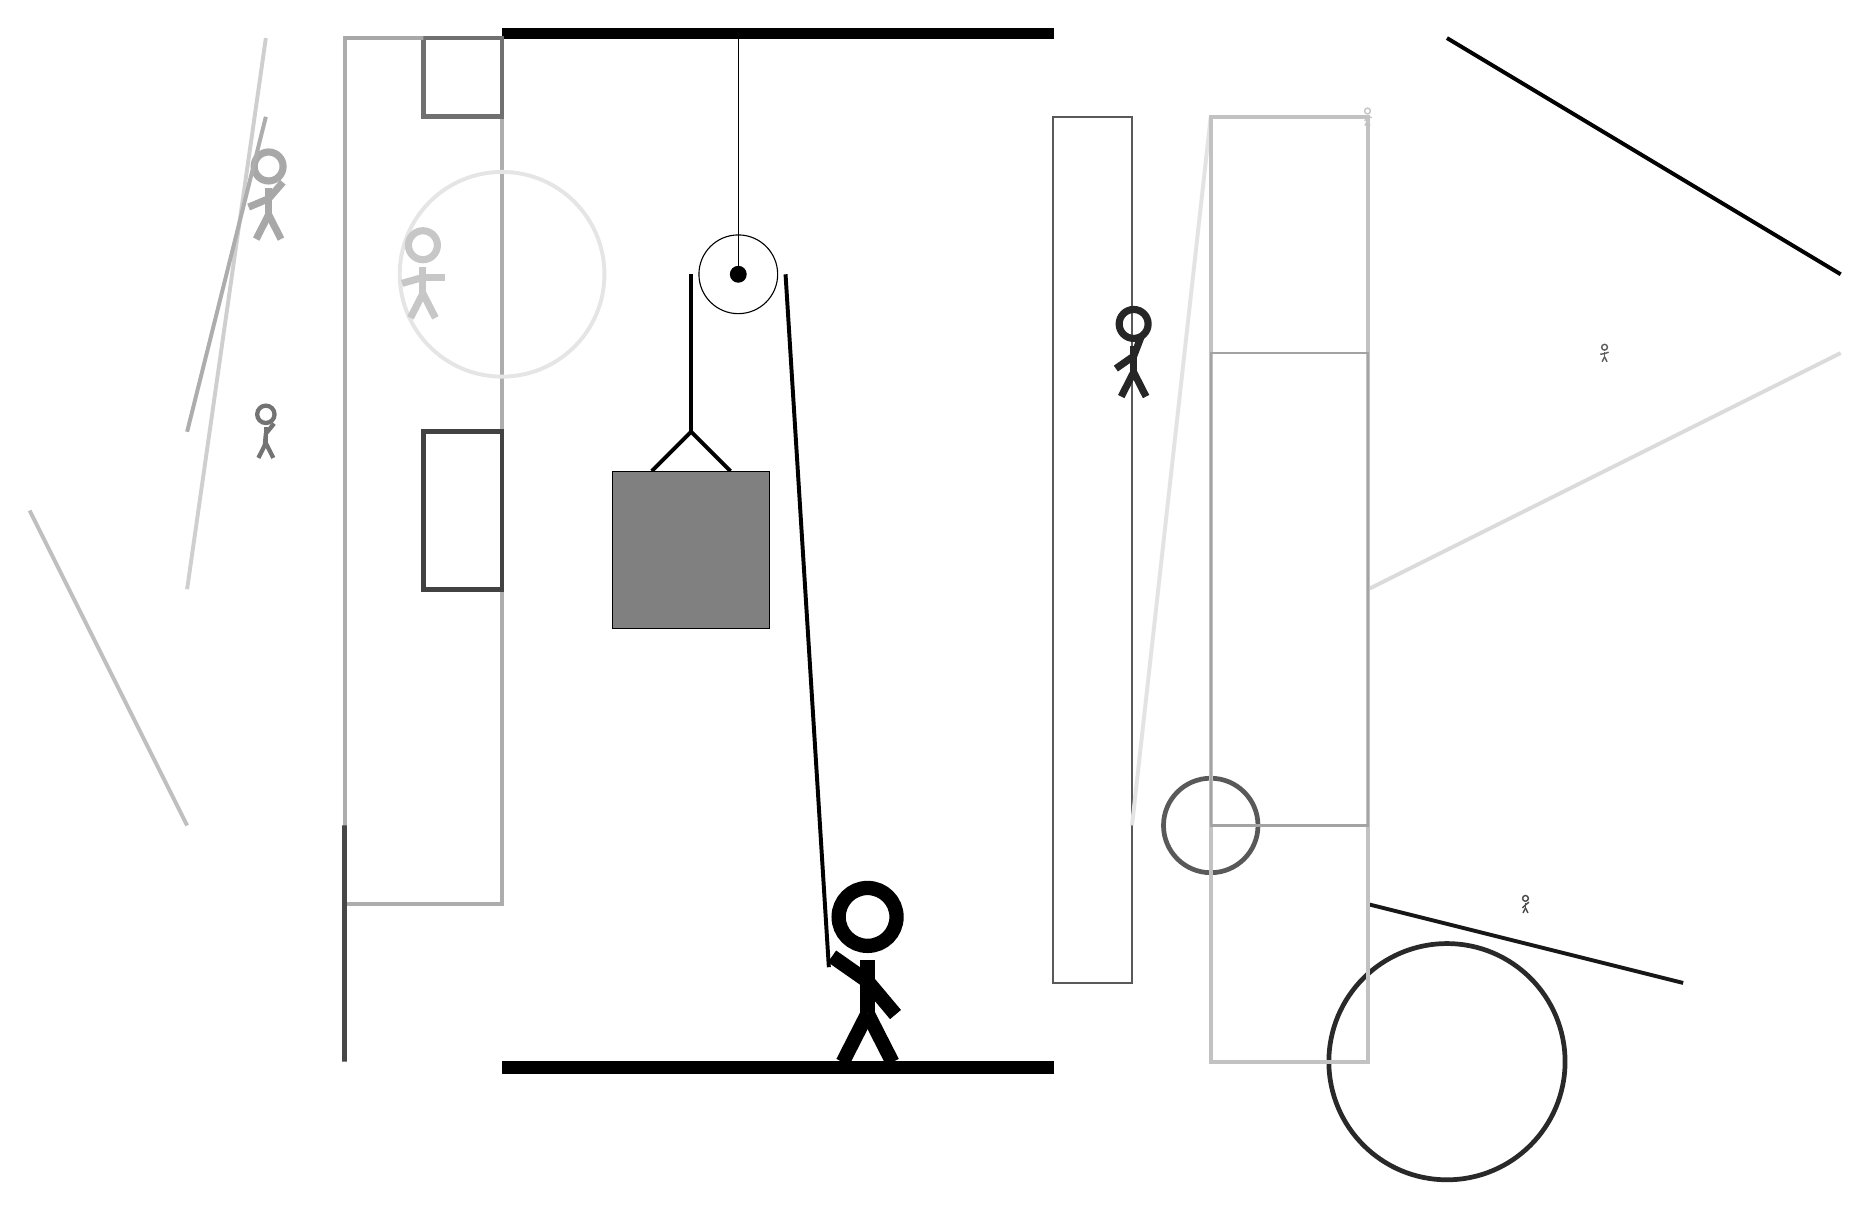
\begin{tikzpicture}
		%%%%% START %%%%%
		
		\draw[fill=black] (-2, 10) rectangle (5, 10.125);
		
		\draw (1, 7) circle (0.5);
		\draw[fill=black] (1, 7) circle (0.1);
		\draw (1, 10) -- (1, 7);
		
		\draw[line width=0.5mm] (-0.1, 4.5) -- (0.4, 5.0) -- (0.9, 4.5);
		\draw[fill=black!50] (-0.6, 4.5) rectangle (1.4, 2.5);
		
		\draw[line width=0.5mm] (0.4, 7) -- (0.4, 5.0);
		\centerarc[line width=0.5mm](1, 7)(0:180:0.6);
		\draw[line width=0.5mm](1.6, 7) -- (2.15, -1.8);
		
		\draw[line width=0.5mm, color=black!14](9, 3) -- (15, 6);
		
		\draw[line width=0.5mm, color=black!91](9, -1) -- (13, -2);
		\draw[line width=0.3mm, color=black!65] (5, -2) rectangle (6, 9);
		\draw[line width=0.5mm, color=black!32] (-2, 10) rectangle (-4, -1);
		
		\draw[line width=0.5mm, color=black!19](-6, 3) -- (-5, 10);
		\draw[line width=0.6mm, color=black!74] (-2, 5) rectangle (-3, 3);
		\node[line width=0.4mm, color=black!34] at (-5, 8) {\Strichmaxerl[5][23][49]};
		\node[line width=0.5mm, color=black!70] at (11, -1) {\Strichmaxerl[1][46][37]};
		\node[line width=0.4mm, color=black!85] at (6, 6) {\Strichmaxerl[5][35][69]};
		\node[line width=0.7mm, color=black!63] at (12, 6) {\Strichmaxerl[1][8][20]};
		\draw [line width=0.6mm, color=black!65](7, 0) circle (0.6);
		
		\draw [line width=0.5mm, color=black!10](-2, 7) circle (1.3);
		\node[line width=0.4mm, color=black!55] at (-5, 5) {\Strichmaxerl[3][85][51]};
		
		\node[line width=0.2mm, color=black!22] at (-3, 7) {\Strichmaxerl[5][16][0]};
		\draw [line width=0.6mm, color=black!84](10, -3) circle (1.5);
		\draw[line width=0.6mm, color=black!56] (-2, 10) rectangle (-3, 9);
		
		\draw[line width=0.4mm, color=black!34] (-3, 10) rectangle (-4, 10);
		
		\draw[line width=0.5mm, color=black!32](-5, 9) -- (-6, 5);
		\draw[line width=0.5mm, color=black!11](6, 0) -- (7, 9);
		
		\draw[line width=0.5mm, color=black!25](-6, 0) -- (-8, 4);
		\draw[line width=0.5mm, color=black!24] (7, 9) rectangle (9, -3);
		\draw[line width=0.6mm, color=black!72] (-4, -3) rectangle (-4, 0);
		\node[line width=0.3mm, color=black!23] at (9, 9) {\Strichmaxerl[1][50][2]};
		\draw[line width=0.5mm, color=black!99](10, 10) -- (15, 7);
		\draw[line width=0.3mm, color=black!36] (7, 6) rectangle (9, 0);
		
		
		\node at (2.6, -1.9) {\Strichmaxerl[10][-35][-50]};
		
		\draw[fill=black] (-2, -3) rectangle (5, -3.15);
		
		%%%%% END %%%%%
	\end{tikzpicture}
\end{document}